\chapter{SISTEMAS EMBARCADOS}
Sistema embarcado em geral é uma combinação de \emph{hardware} e \emph{software} para executar uma tarefa específica diferente dos computadores do dia-a-dia que possuem inúmeros propósitos: verifica e-mail, escrever monografias, entre outros. Sistemas embarcados podem possuir ou não um sistema operacional, seja um RTOS, possui requisitos de tempo de execução, ou um Linux e, portanto, pode ser desenvolvido em um \emph{hardware} com microcontrolador ou microprocessador \cite{wikibook2012embedded}.

Segundo \cite{cunha2013} a inteligência embarcada é uma tendência futura, cada vez mais inteligência será adicionada aos equipamentos do dia-a-dia, considera que um microondas atual tem mais capacidade computacional do que tinha o projeto Apolo, que levou o homem a lua. Esta crescente utilização se dá basicamente pelo preço e consumo reduzido dos microcontroladores, além da grande flexibilidade ao atender os mais diversos problemas visto o vasto número de arquiteturas disponíveis: ARM, MIPS, Coldfire/68k, PowerPC, x86, PIC, 8051, Atmel AVR, Renesas H8, SH, V850, FR-V, M32R, Z80, Z8 e outras. Um contraste que atrai diversos desenvolvedores quando comparado com o número limitado de arquiteturas diponíveis para microprocessadores do mercado de computadores pessoais \cite{germano2011}.

A comunicação dos microcontroladores com o meio externo, segundo \cite{germano2011}, se dá pelos periféricos e o mais comuns são:
\begin{itemize}
\item Entrada de dados através de teclas (geralmente através de teclados feitos com varredura matricial);
\item Leds;
\item Display’s de LCD (sendo os mais comuns os alfanuméricos por exemplo o HD44780);
\item Interface serial – (Por exemplo RS 232, I2C);
\item Universal Serial Bus – (USB);
\item TCP/IP.
\end{itemize}

Como dito anteriormente, esses sistemas estão cada vez mais no dia-a-dia das pessoas e, claro, facilitando a vida delas, mas muitas vezes não são percebidos. E cada vez mais estão mais acessíveis podendo automatizar funções até mesmo dentro das próprias casas. A Figura \ref{fig:exemplosistemasembarcados}\footnote{\url{http://bytesdontbite.com/2012/06/26/embedded-systems-no-bdb/}} mostra alguns sistemas embarcados e onde são utilizados:

\begin{figure}[htp]
	\centering
	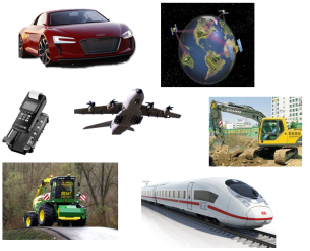
\includegraphics[scale=1]{images/exemplo_sistemas_embarcados.png}
	\caption{Exemplo de Sistemas embarcados}	
	\label{fig:exemplosistemasembarcados}	
\end{figure}

\section{SISTEMAS EMBARCADOS DE TEMPO}
O conceito Tempo Real é complexo para ser explicado, mas sua ideia básica é que se espera que o computador responda algo para o ambiente externo em tempo. Normalmente pessoas assumem que tempo real significa “muito rápido”, entretanto não é verdade, tempo real simplesmente significa “rápido o suficiente” no contexto de operação do sistema. Um exemplo é a ação do motor, pode-se dizer que é “rápida”, pois o sistema deve tomar decisões como - fluxo de combutível, tempo da faísca - toda vez que o motor completa um ciclo.

Sistemas de tempo real são baseados em previsibilidade e, segundo \cite{farines2000sistemas}, essa previsibilidade de um sistema de tempo real é obtida quando independente de falhas, sobrecargas e variações de hardware, e assim é possível que seu comportamento seja antecipado antes de sua execução. Isso tem a finalidade de poder prever o funcionamento de um sistema de tempo real e garantir as suas restrições temporais, e para isso é necessário definir hipóteses em relação a carga e falhas em relação ao ambiente externo deste sistema \cite{farines2000sistemas}. 
Segundo \cite{mall2009real} os sistemas de tempo real são classificados em dois tipos:
\begin{itemize}
\item \emph{Soft Real Time Systems}: Sistemas não críticos de tempo real, onde a ocorrência de uma falha temporal é da mesma ordem de grandeza que os resultados em que o funcionamento está correto, exemplos: Máquina de lavar e portão eletrônico de uma casa;
\item \emph{Hard Real Time Systems}: Sistemas Críticos de Tempo Real, onde a ocorrência de uma falha temporal complicam, e muito, os resultados quando comparado com seu funcionamento correto, exemplos: sistema de controle de um avião e um sistema de controle de semáforos.
\end{itemize}

\section{SISTEMAS EMBARCADOS CRÍTICO}
\label{sec:SistemaEmbarcado}

Sistema Crítico é um sistema no qual a confiança é fundamental, ou melhor, a questão mais importante em seu desenvolvimento. Isso porque sistemas críticos, em caso de falha, podem causar consequências gravíssimas para os humanos, economia e outras áreas. Pode-se dizer que seus indicadores são: Disponibilidade, confiabilidade, segurança e proteção. E para que essa confiança seja alcançada deve-se evitar erros durante seu desenvolvimento e realizar diversos testes para que seja possível detectar e corrigir os erros que passarem de forma que seja possível limitar os danos causados por falhar operacionais \cite{sommerville2004software,feldmann2007survey,jordan2006standard}.

Segundo \cite{kopetz2011real} as classificações dos sistemas embarcados críticos podem ser:
\begin{itemize}
\item \emph{Fail Safe}: Classficação para sistemas onde o estado seguro pode ser atingido em caso de falha, como por exemplo, esgotar a bateria de uma bomba de insulida;
\item \emph{Fail Operational}: Classificação para sistemas que em caso de falhas ainda são capazes de fornecer algum tipo de serviço, mesmo que mínimo. Um exemplo é um sistema de controle de vôo que, mesmo em caso de falha, é capaz de fornecer serviços e ser seguro.
\end{itemize}

Abaixo a Figura \ref{fig:exSistEmbarcado},  mostra exemplos de sistemas embarcados críticos.

\begin{figure}[htp]
	\centering
	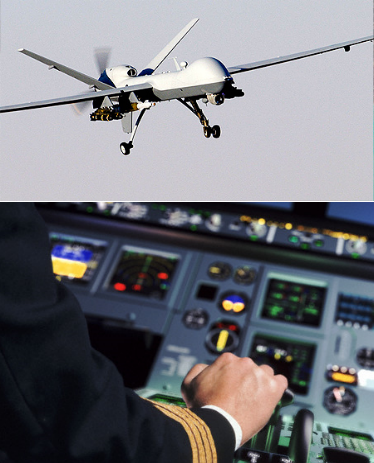
\includegraphics[scale=0.7]{images/exemplo_sistemas_embarcados_criticos.png}	
	\caption{Sistemas embarcos críticos}
	\label{fig:exSistEmbarcado}	
\end{figure}

\section{MICROCONTROLADOR}
Microcontroladores são chips inteligentes que utilizam a arquitetura Harvard, RISC. É constituído basicamente por pinos de entradas e saídas e memória. Suas saídas podem ser controladas através de programação e em função do processamento de suas entradas. Sua programação pode ser feita em diversas linguagens como: C, C++, entre outras \cite{radio2012amadores}.

Segundo \cite{ganssle1999art}, o microcontrolador é a parte mais importante de um sistema embarcado e sua principal diferença quando comparada com um microprocessador é o fato de ser um sistema computacional completo que integra todos as principais partes da arquitetura de Von Neumann em um único componente, as partes citadas são:
\begin{itemize}
\item CPU: \emph{Central Processor Unit};
\item Memória RAM: \emph{Random Access Memory};
\item Portas I/O: Portas de entrada e saída.
\end{itemize}

Além de ser composto por temporizadores, memória ROM (\emph{Read Only Memory}), conversor AD, analógico – digital, e DA, digital – analógico.
Comparados com microprocessadores, os microcotroladores possuem consumo e clock, processamento, reduzidos, isso devido ao fato que o primeiro é destinado a tarefas que necessita uma alta capacidade de processamento como, por exemplo, os microprocessadores dos nossos desktop do dia-a-dia. Por padrão, os microprocessadores são utilizados em situações que os requisitos são abrangentes, com entradas e saída variadas como: sensores, atuadores e periféricos de comunicação \cite{lee2011introduction}.

\subsection{PIC}
PIC é um circuito integrado produzido pela \emph{Microchip Technology Inc}. Seu nome significa: \emph{Programmable Interface Controller}, Controlador de Interface Programável. Externamente possui uma aparência de um circuito integrado mais comuns - TTL ou CMOS -, mas na verdade contém todos os componentes de um sistema microprocessado como: CPU, \emph{Central Processor Unit}, sua finalidade é interpretar as instruções de programa; Memória PROM, \emph{Programmable Read Only Memory}, na qual memorizará as instruções do programa; Memória RAM, \emph{Random Access Memory}, utilizada pra memorizar as variáveis do programa; Linhas de I/O, entrada e saída, para controlar dispositivos internos e receber informações do meio externo; entre outros \cite{radio2012amadores,wikipedia2012pic}.

\subsection{SENSORES}
A definição de sensor pode ser a de um transdutor capaz de alterar sua característica física interna em resposta à um fenômeno físico externo. Além disso, existem sensores considerados de operação indireta que são os quais alteram suas propriedades como capacitância, resistência, ou, até mesmo, sua indutância, sob ação de algum gradeza ou evento externo \cite{rosario2006principios}. 

Segundo \cite{nomadusp2014}, os sensores são largamente utilizados na medicina, indústria, robótica, além de outras aplicações. Considerando que o sinal é sempre uma forma de energia, os sensores podem ser classificados em função da energia que é capaz de detectar, como:

\begin{itemize}
\item Sensores de luz: células solares, fotodíodos, fototransistores, tubos fotoelétricos, e outros;
\item Sensores de som: microfones e hidrofone;
\item Sensores de temperatura: termômetros e termopares;
\item Sensores de resistência elétricas: ohmímetro. 
\item Outros;
\end{itemize}

\subsection{SENSORES BIOLÓGICOS}
Segundo \cite{nomadusp2014}, os sensores citados anteriormente são corretamente chamados de sensores artificiais. Isto devido ao fato de existir sensores naturais ou biológicos, já que todos os organismos vivos possuem sensores capazes de agir da mesma forma que os sensores artificias. Esses sensores biológicos são células especializadas, sensíveis a:

\begin{itemize}
\item Luz, movimento, temperatura, vibração, pressão, campos eléctricos, som, e outros aspectos físicos do ambiente;
\item Grande variedade de moléculas ambientais, incluindo toxinas e nutrientes;
\item Aspectos metabólicos, tais como os níveis de glicose e oxigênio;
\item Até mesmo as diferenças entre proteínas do ambiente externo e do próprio organismo.
\end{itemize}

Esses sensores artificiais que imitam sensores biológicos, utilizando componentes biológicos, são chamados biossensores.

\subsection{ATUADORES}
Segundo \cite{chironis1991mechanisms}, dispositivos considerados atuadores são aqueles que transformam uma forma de energia em outra, causando mudanças no ambiente em que estão atuando, ou seja, de acordo com sinais, ou impulsos, recebidos realizam ações capazes de alterar as grandezas físicas do ambiente em questão. Eles são capazes de converter energias como: energia elétrica, hidráulica e pneumática em energia mecânica. Segue exemplos de alguns tipos de atuadores:

\begin{itemize}
\item Atuadores eletromagnéticos: São os motores elétricos como motores de passos, servos;
\item Atuadores hidráulicos: Utilizam um fluido submetido a uma pressão para movimentar um braço, são utilizados em robô que operam grandes cargas;
\item Atuadores pneumáticos: Utilizam um gás submetido a uma pressão para movimentar o braço, possuem menor custo que os hidráulicos, sendo utilizados em robôs de menor porte;
\end{itemize}

\subsection{MOTOR DE PASSO}
Motor de passo é um dispositivo eletromecânico. Sua principal propriedade é sua habilidade de transformar pulsos elétricos em movimentos, esses movimentos são precisamente incrementados na posição do rotor e são denominados ‘passos’. Esse tipo de motor é caracterizado como máquina duplamente saliente, o que significa que possui dentes, compostos por matérias magnéticos nas duas partes que o compõe: A parte imóvel chamada estator e a móvel rotor \cite{demotor, acarnley2002stepping}.

Seu uso é interessante em situações em que precisão nos movimentos é necessária. Isso porque com ele é possível controlar: ângulo de rotação, velocidade, posição e sincronismo. Suas vantagens não são seu torque nem a capacidade de gerar movimentos de alta velocidade, mas sim a precisão em seus movimentos. Devido a essas características esse tipo de motor é amplamente utilizado em: câmeras de vídeo, robôs, brinquedos, scanners, impressoras, entre outros \cite{demotor}.

De forma simples o funcionamento de um motor de passo consiste no uso de materiais magnéticos, ou solenoides, como dito anteriormente, alinhados dois a dois, representando os polos norte e sul, que quando energizados atraem o rotor fazendo-o se alinhar as partes energizadas do estator, causando assim um pequeno movimento: o passo. Sua velocidade e sentido estão diretamente relacionados à forma com que os solenoides são acionados, o primeiro com a frequência e o segundo a ordem de acionamento \cite{demotor, acarnley2002stepping,wikipedia2012stepper}.

\subsection{MOTOR DE PASSO RELUTÂNCIA VARIÁVEL – \emph{MULTI STACK}}
A fonte do fluxo magnético desse tipo de motor são as bobinas colocadas nos dentes do estator. O acionamento das bobinas é feito em sequência para incentivar o movimento, alinhamento, dos conjuntos de dentes sucessivos do estator e do rotor dando ao motor a característica de passos. Ao longo de eu eixo ele é dividido em seções isoladas magneticamente chamadas \emph{stacks}, daí o nome \emph{multi stack}, e cada uma pode ser excitada por uma bobina separadamente chamada phase. Cada \emph{stack} possui um estator, preso em sua posição pela caixa, suporte, do motor junto com as bobinas e o elemento móvel, rotor.

O rotor é uma unidade única e maciça que será utilizado para a movimentação da carga. O material do rotor é um metal elétrico laminado o que permite que o campo magnético possa mudar rapidamente sem grandes perdas. O estator de cada rotor possui um determinado número de polos e uma parte da \emph{phase}, bobina, é enrolada em torno de cada polo para produzir o campo magnético. Os polos adjacentes são enrolados no sentido oposto assim os campos magnéticos adjacentes possuem sentidos opostos. Com isso o circuito magnético completo é considerado um polo do estator, o dente do rotor, o vão de ar entre os dentes de ambos e, por fim, um polo adjacente do estator. E esse circuito é repetido a cada par de polos do estator. As forças normais produzidas pelos polos do estator e os dentes do rotor são iguais e se anulam assim sobra apenas a força tangencial o que causa o movimento, isso pode ser visto conforme a Figura ~\ref{fig:forcamotorpassobainfusao}.

\begin{figure}[htp]
	\centering
	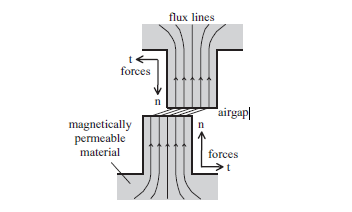
\includegraphics[scale=1]{images/forca_motor_passo.png}
	\caption{Forças normais e tangenciais}	
	\label{fig:forcamotorpassobainfusao}	
\end{figure}

A posição do rotor com relação ao estator é ajustada toda vez que as bobinas são excitadas. O ajuste ocorre, pois os dentes de ambos são alinhados o que tende a diminuir a relutância do circuito magnético, daí surgiu o nome do motor. Considerando a Figura ~\ref{fig:visaomotorpasso} é possível perceber que para girar no sentido horário a ordem de acionamento deve ser A, B, C, A, B, C, A... e no sentido anti-horário A, C, B, A, C, B, A...

\begin{figure}[htp]
	\centering
	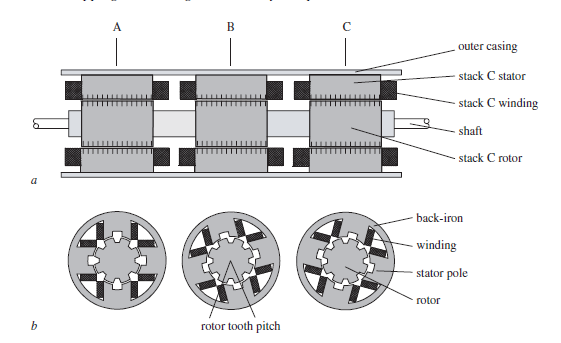
\includegraphics[scale=1]{images/visao_motor_passo.png}
	\caption{Visão paralela e perpendicular das \emph{stacks} e rotor}	
	\label{fig:visaomotorpasso}	
\end{figure}

\newpage Segundo \cite{acarnley2002stepping}, existe uma pequena relação entre o comprimento do passo. Considere N o número de dentes do estator e p o número de dentes do rotor logo: 

\begin{equation}
  \emph{step length} = 360/(N * p)
\end{equation}

\subsubsection{\emph{DESIGN} DO MOTOR}
Cada polo do estator produz um campo magnético quando excitado com uma corrente DC. A performance do motor depende da força do campo magnético gerado pelas bobinas quando excitadas, logo o campo magnético está diretamente ligado ao torque do motor. A força do campo magnético está relacionada à intensidade da corrente que passa pelas bobinas, portanto em teoria aumentar a corrente para aumentar o torque seria o suficiente, entretanto existe um limitante que é o aumento da temperatura nas bobinas.

No exemplo da Figura ~\ref{fig:visaomotorpasso} cada \emph{stack} tem 4 polos. Uma vez que todas as quatro bobinas devem ser excitadas concorrentemente uma prática comum é interconectar as bobinas para formar apenas uma \emph{phase}. A forma com que as bobinas são interconectadas influência na temperatura que será dissipada pela bobina uma vez que isso está diretamente ligada à intensidade da corrente. A potência não varia conforme a interconexão. 

Existem 3 formas de interconexão conforme a Figura ~\ref{fig:bobinas}. Na verdade a potência não varia conforme a interconexão, mas sim qual \emph{driver} de controle será utilizado: baixa voltagem e alta corrente com uma conexão paralela ou alta voltagem e baixa corrente com uma conexão em série. A diferença entre as 3 interconexões pode ser vista na Figura ~\ref{fig:relacaobobina} \cite{acarnley2002stepping}.

\begin{figure}[htp]
	\centering
	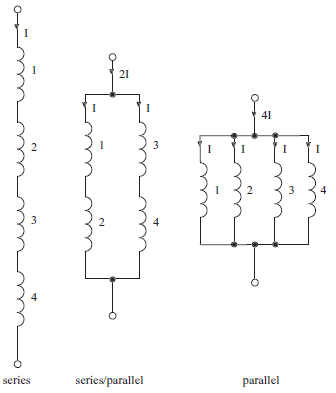
\includegraphics[scale=1]{images/bobinas.png}
	\caption{Interconexão das bobinas}	
	\label{fig:bobinas}	
\end{figure}

\begin{figure}[htp]
	\centering
	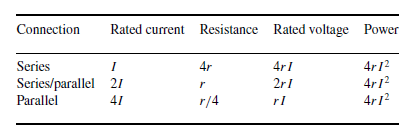
\includegraphics[scale=1]{images/relacao_bobina.png}
	\caption{Relação das interconexões das bobinas}	
	\label{fig:relacaobobina}	
\end{figure}

\subsection{MOTOR DE PASSO RELUTÂNCIA VARIÁVEL – \emph{SINGLE STACK}}
Como o nome já diz esse motor é construído com apenas uma stack, ou melhor, uma unidade. Entretanto quanto ao funcionamento e princípios básicos é idêntico ao \emph{multi stack}. Cada dente do estator ainda possui uma bobina separada que produz um campo magnético quando excitada por uma corrente DC.

Uma mudança é que as bobinas do lado oposto são conectadas para formar uma phase. Na Figura ~\ref{fig:singlestack} existe 3 phases que é o número mínimo para poder rotacionar para os dois lados. A bobina no dente oposto no estator está no sentido oposto para que sejam gerados campos magnéticos em sentidos opostos. E por fim a relação de comprimento do passo se mantém conforma o motor \emph{multi stack} \cite{acarnley2002stepping}.

\begin{figure}[htp]
	\centering
	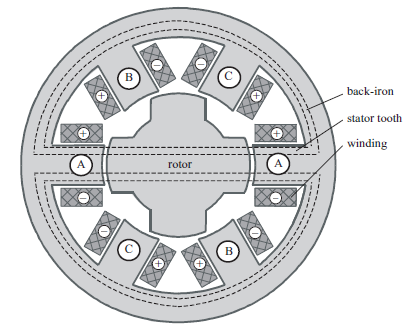
\includegraphics[scale=1]{images/single_stack.png}
	\caption{\emph{Stator single stack}}	
	\label{fig:singlestack}	
\end{figure}

\subsection{MOTOR DE PASSO HÍBRIDO}
A diferença principal desse com os tipos anteriores é que o circuito magnético é excitado por uma combinação de bobinas e imã permanente. Seu funcionamento e princípios básicos são idênticos ao \emph{multi} e \emph{single stack}. As bobinas ainda permanecem nos dentes do estator já o imã compõe o eixo do rotor conforme Figura ~\ref{fig:hibrido}.

\begin{figure}[htp]
	\centering
	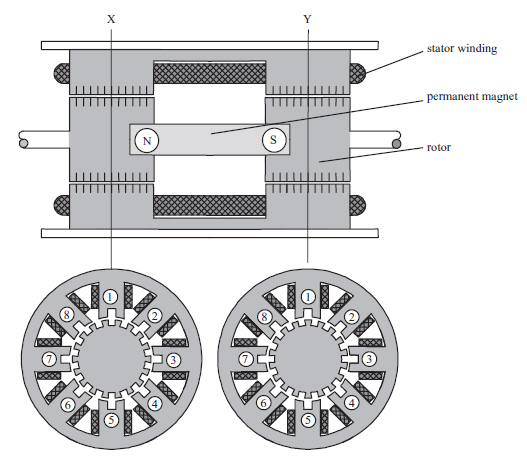
\includegraphics[scale=0.7]{images/hibrido.png}
	\caption{Motor híbrido}	
	\label{fig:hibrido}	
\end{figure}

Existem duas bobinas, \emph{phases}, situadas em 4 dos 8 polos do estator, conforme Figura \ref{fig:hibrido}. A bobina A está nos polos 1, 3, 5, 7 e a B nos polos 2, 4, 6, 8. Polos adjacentes ainda são envolvidos pelas bobinas em sentidos opostos, portanto se a bobina A é alimentada com corrente positiva o campo magnético é direcionado para fora nas bobinas 3 e 7, mas para dentro nos polos 1 e 5 e o mesmo acontece na bobina B.

Quando se aplica corrente nas bobinas a mesma ideia de alinhamento dos dentes do rotor e stator acontece. Considerando a Figura \ref{fig:hibrido} e o exemplo da excitação positiva na bobina A, citada anteriormente, o estator e o rotor são alinhados sob os polos 3 e 7 na seção X e polos 1 e 4 na seção Y.

Para uma rotação continua o motor necessita de uma excitação sequencial das bobinas. Se retirar a excitação de A e colocar em B o alinhamento dos dentes vai acontecer com 4 e 8 na seção X e 2 e 6 na seção Y. Isso faz com que o motor gire no sentido horário, a sequência deve ser A+, B+, A-, B-,... Para o sentido anti-horário A+, B-, A-, B+.

Segundo \cite{acarnley2002stepping}, a relação de comprimento do passo é similar ao de relutância variável. Existe uma relação com o número de dentes do rotor p, e com um ciclo completo de excitação. Como um esse ciclo em um motor hibrido consiste em 4 estados e produz 4 passos de movimento no rotor, logo conclui-se que:
\begin{equation}
  \emph{step length} = 360/(4 * p) = 90 / p
\end{equation}

\subsection{COMPARAÇÃO ENTRE TIPOS DE MOTORES}
Não é possível dizer categoricamente que um motor é melhor do que o outro em todas as situações. Os híbridos têm menor comprimento de passo, normalmente 1,8 graus, o que pode ser uma grande vantagem quando alta precisão é necessária. Eles também possuem maior torque devido ao uso do imã permanente no rotor. E, além disso, quando nenhuma bobina esta excitada o motor hibrido ainda possui um "torque de retenção" que mantém a posição do rotor. E isso pode ser uma característica na aplicação onde a posição do rotor deve ser preservada durante uma falha de energia, mas é bom lembra que esse torque é menor do que o torque com 1 ou mais bobinas excitadas.

Já o de relutância variável tem duas vantagens quando se trata de movimentar carga em distâncias consideráveis. A primeira é que tipicamente o comprimento de seu passo é de 15 graus, maior que o do híbrido, portanto ele precisa de menos passos para mover a mesma distância. Com a redução do número de excitações das bobinas o consumo também é reduzido, em caso de uso de baterias é uma característica muito interessante. A segunda é que por não possuir imã permanente possui uma menor inércia para início de movimento, também diminuindo o consumo inicial \cite{acarnley2002stepping}.

\subsection{LCD - \emph{Liquid Crystal Display}}
